\lab{HIV Treatment Using Optimal Control}{HIV Treatment Using Optimal Control}
\label{lab:hiv}
\labdependencies{NumericalIVP}

\section*{Introduction}
Viruses cause many common illnesses in society today, including influenza, the common cold, and COVID-19.
Viruses are obligate parasites, meaning that they must infect a host in order to replicate.
After entering a host cell, viruses hijack host machinery to replicate their genome and translate their proteins.
After this process, the new virus particles are assembled and lyse (break apart) the host cell to find a new host.

Mammalian immune systems are composed of two interconnected systems: the innate immune system and the adaptive immune system.
While both branches of the immune system can combat viruses, the adaptive immune system is especially suited to recognize and neutralize viral infections.
A major part of the adaptive immune response is helper T cells, as these cells moderate and regulate all other facets of the immune response.
Helper T cells are most characterized by the presence of a receptor called CD4, which helps the cell recognize infections.

One of the most devastating viral illnesses today is acquired immunodeficiency syndrome (AIDS), caused by the human immunodeficiency virus (HIV).
HIV specifically targets and replicates in helper T cells, rendering them nonfunctional and killing them.
By taking out the most important regulator of the immune system, HIV makes it difficult for the body to fight infection, so sicknesses that would normally be trivial for the body to manage, such as the common cold, yeast infections, and pneumonia, become deadly.

Currently, there is no cure for HIV, and vaccines are difficult to develop.
Treatments that curb the replication of HIV and help maintain healthy helper T cell population levels are available, but they are expensive and must be taken for the rest of a patient's life.
Optimizing the dosage is essential to maximize the drug's effect while minimizing the cost and negative side-effects of long-term usage.
In this lab, we will use optimal control to find the optimum dosage of a two-drug combination to fight HIV.
In this lab we will use optimal control to find the optimal dosage of a two-drug combination\footnote{\textit{SHORT COURSES ON THE MATHEMATICS OF BIOLOGICAL COMPLEXITY}, Web. 15 Apr. 2015 http://www.math.utk.edu/~lenhart/smb2003.v2.html.}.

\section*{Derivation of Control}
We begin by defining some variables.
Let

\begin{itemize}
    \item $T$ represent the concentration of CD4$^+$ T cells,
    \item $V$ the concentration of HIV particles,
    \item $s_1$ and $s_2$ the production of T cells by various processes,
    \item $B_1$ and $B_2$ the half saturation constants (like crowd control in the blood stream and plasma),
    \item $\mu$ the death rate of uninfected T cells,
    \item $k$ the rate of infection of T cells,
    \item $c$ the death rate of the virus,
    \item $g$ the input rate of some external viral source, and
    \item $u_1$ and $u_2$ the control variables, corresponding to the amount of drugs that introduce new T cells or kill the virus, respectively.\footnote{`Immunotherapy of HIV-1 Infection', Kirschner, D. and Webb, G. F., Journal of Biological Systems, 6(1), 71-83 (1998)}
\end{itemize}

Next we write the state system, the equations that describe the changes in T cells and viruses:\footnote{`Optimal Control of an HIV Immunology Model', H.R Joshi}

\begin{equation}
	\begin{alignedat}{2}
		\frac{\it{d}T(t)}{\it{dt}} &= s_1 - \frac{s_2V(t)}{B_1+V(t)} - \mu T(t)-kV(t)T(t)+u_1(t)T(t), \quad & T(0) &= T_0, \\
		\frac{\it{d}V(t)}{\it{dt}} &= \frac{gV(t)}{B_2+V(t)}\big(1-u_2(t)\big) - cV(t)T(t), & V(0) &= V_0.
	\end{alignedat}
    \label{eq:hiv:state}
\end{equation}
The term $s_1-\frac{s_2V}{B_1+V}$ is the source/proliferation of unaffected T cells, $\mu T$ the natural loss of T cells, $kVT$ the loss of T cells by infection, $\frac{gV}{B_2+V}$ the viral contribution to plasma, and $cVT$ the viral loss.

We now seek to maximize the functional 
\[
J(u_1,u_2) = \int_0^{t_f}[T-(A_1u_1^2+A_2u_2^2)]\it{dt}.
\]
This functional considers (1) the benefit of T cells, and (2) the systematic costs of drug treatments.
The constants $A_1$ and $A_2$ represent scalars to adjust the size of terms coming from $u_1^2$ and $u_2^2$ respectively.
We seek an optimal control $u_1^*,u_2^*$ satisfying
\[
J(u_1^*,u_2^*)=\max_{(u_1,u_2)\in U}J(u_1,u_2) =\min_{(u_1,u_2)\in U}-J(u_1,u_2),
\]
where $U=\{(u_1,u_2):\,a_i\le u_i(t) \le b_i\text{ for }t\in[0,t_f], i=1,2\}$.
 
\section*{Optimality System}
The Hamiltonian is defined as:
\begin{align*}
	H = \vec{\lambda} \cdot \vec{f} - L\\
	H =\lambda_1\left[ s_1 - \frac{s_2V}{B_1+V}-\mu T-kVT+u_1T \right] &+ \lambda_2 \left[\frac{g(1-u_2)V}{B_2+V}-cVT\right]\\
	 &+  \left[T-(A_1u_1^2+A_2u_2^2)\right].
\end{align*}
Note that the costate is represented with $\lambda$ instead of $p$.
The costate evolution equations are:
\begin{equation}
    \begin{alignedat}{2}
        \lambda_1^{'} &=-\frac{\partial H}{\partial T} =  -1+\lambda_1[\mu+kV-u_1]+\lambda_2cV, & \lambda_1(t_f) &= 0, \\
        \lambda_2^{'} &= -\frac{\partial H}{\partial V} = \lambda_1\left[\frac{B_1s_2}{(B_1+V)^2}+kT\right] -\lambda_2\left[\frac{B_2g(1-u_2)} {(B_2+V)^2}-cT\right], \quad & \lambda_2(t_f) &= 0.
    \end{alignedat}
    \label{eq:hiv:costate}
\end{equation}
Using Pontryagin's maximum principle to find the control, we have
\begin{equation*}
\frac{\partial H}{\partial u_1} = -2A_1u_1(t)+\lambda_1T(t)=0 \hspace{1.5cm}
\frac{\partial H}{\partial u_2} = -2A_2u_2(t)+\lambda_2\left[\frac{-gV(t)}{B_2+V(t)}\right]=0
\end{equation*}
which gives (provided these are within the bounds of the controls)
\begin{align*}
	u_1^*(t) &= \frac{1}{2A_1}\left[\lambda_1T(t)\right],\\
	u_2^*(t) &= \frac{-1}{2A_2}\left[\lambda_2\frac{gV(t)}{B_2+V(t)}\right].
\end{align*}
Taking into account the bounds on the controls, we have
\begin{align}
	\begin{split}
		u_1^*(t)&=\min\left\{\max\{a_1,\frac{1}{2A_1}(\lambda_1T(t))\},b_1\right\},\\
		u_2^*(t)&=\min\left\{\max\{a_2,\frac{-\lambda_2}{2A_2}\frac{gV(t)}{B_2+V(t)}\},b_2\right\}.
	\end{split}
    \label{eq:hiv:optimal_control}
\end{align}

\section*{Creating a Numerical Solver}

In the preceding derivation, the states, costates, and controls all depend on each other, so we can't just solve the system once, not even numerically.
Instead we must iteratively solve for the control $u$.
In each iteration we solve our state equations and our costate equations numerically, then use those to find our new control.
Lastly, we check to see if our control has converged.
To solve each set of differential equations, we will use \li{solve_ivp}.
However, our state equations depend on $u$, our costate equations depend on our state equations, and both depend on a lot of constants.
Therefore, we will define \li{state_equations} and \li{costate_equations} to accept these as additional arguments, and we will give these additional arguments to \li{solve_ivp} with the \li{args} keyword.

We'll use the following constants throughout this lab:

\begin{lstlisting}
# Constants used in equations
a_1, a_2 = 0, 0
b_1, b_2 = 0.02, 0.9
s_1, s_2 = 2, 1.5
mu = 0.002
k = 0.000025
g = 30
c = 0.007
B_1, B_2 = 14, 1
A_1, A_2 = 250000, 75

constants = a_1, a_2, b_1, b_2, s_1, s_2, mu, k, g, c, B_1, B_2, A_1, A_2

# Other constants
T0, V0 = 400, 3
n = 2000
t_f = 50
\end{lstlisting}

\begin{problem}
Create a function that defines the state equations as in \eqref{eq:hiv:state} and returns both equations in a single array.
The function should be able to be passed into \li{solve_ivp}.

\begin{lstlisting}
def state_equations(t, y, u_interpolation, constants):
    '''
    Parameters
    ---------------
    t : float
        the time
    y : ndarray (2,)
        the T cell concentration and the virus concentration at time t
    u_interpolation : CubicSpline
        the values of the control u_interpolation(t) = [u1(t), u2(t)]
    constants : a_1, a_2, b_1, b_2, s_1, s_2, mu, k, g, c, B_1, B_2, A_1, A_2
    
    Returns
    --------------
    y_dot : ndarray (2,)
        the derivative of the T cell concentration and the virus concentration at time t
    '''

    a_1, a_2, b_1, b_2, s_1, s_2, mu, k, g, c, B_1, B_2, A_1, A_2 = constants
\end{lstlisting}

You may use the following code to check that your function implements the state equations correctly:

\begin{lstlisting}
u = lambda _: np.full(2, 1/2)
state = np.ones(2)

state_equations(0, state, u, constants)
# This should result in [2.397975, 7.493].
\end{lstlisting}

\label{problem:hiv:state}
\end{problem}

\begin{problem}
Create a function that defines the costate equations as in \eqref{eq:hiv:costate} and returns both equations in a single array.
The function should be able to be passed into the \li{solve_ivp}.

\begin{lstlisting}
def costate_equations(t, y, u_interpolation, state_solution, constants):
    '''
    Parameters
    ---------------
    t : float
        the time
    y : ndarray (2,)
        the lambda values at time t 
    u_interpolation : CubicSpline
        the values of the control u_interpolation(t) = [u1(t), u2(t)]
    state_solution : result of solve_ivp on state_equations with
        dense_output=True, i.e., state_solution.sol(t) = [T(t), V(t)]
    constants : a_1, a_2, b_1, b_2, s_1, s_2, mu, k, g, c, B_1, B_2, A_1, A_2
    
    Returns
    --------------
    y_dot : ndarray (2,)
        the derivative of lambda at time t
    '''

    a_1, a_2, b_1, b_2, s_1, s_2, mu, k, g, c, B_1, B_2, A_1, A_2 = constants
\end{lstlisting}

You may use the following code to check that your function implements the costate equations correctly:

\begin{lstlisting}
u = lambda _: np.full(2, 1/2)
costate = np.ones(2)
class test_state_solution(): sol = lambda self, _: np.ones(2)

costate_equations(0, costate, u, test_state_solution(), constants)
# This should result in [-1.490975, -3.64964167].
\end{lstlisting}

\label{problem:hiv:costateequations}
\end{problem}


\begin{figure}
\centering
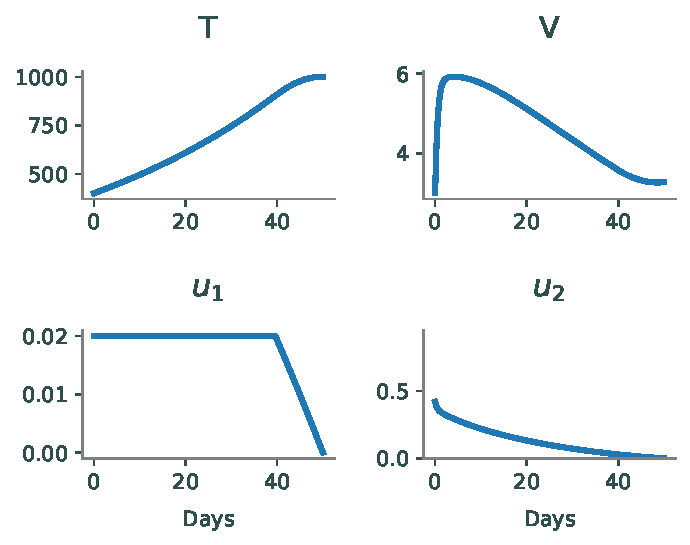
\includegraphics[width=5in]{figures/hiv_solution.pdf}
\caption{The solution to Problem \ref{problem:hiv:numericalsolver}.}
\label{fig:hiv:solutions}
\end{figure}

Finally, we can put these together to create our solver.
\begin{problem}
Create and run a numerical solver for the HIV two drug model using the code below.
Use \eqref{eq:hiv:optimal_control} to solve for $u_1^*$ and $u_2^*$.

Note that while the state equations have initial conditions, the costate equations have end conditions.
Fortunately \li{solve_ivp} can handle this by reversing the start and end time arguments and then making sure to index the results backwards.
For example, you might use \li{<solve_ivp_result>.y[:, ::-1]}.

When using \li{solve_ivp}, specify \li{max_step=0.5} to help with convergence, and make sure you're using the Runge--Kutta algorithm (\li{method="RK45"}).
Also set \li{dense_output=True} so that you can call \li{<solve_ivp_result>.sol(t)} at arbitrary values of $t$ in your state and costate equations.
Finally, use \li{np.linspace(0, t_f, n)} for the \li{CubicSpline} interpolation of $u$ and to evaluate \li{state_solution} and \li{costate_solution} when solving for the next $u_1$ and $u_2$.

\begin{lstlisting}
# Initialize state, costate, and u.
state0 = np.array([T0, V0])
costate0 = np.zeros(2)

u = np.zeros((2, n))
u[0], u[1] = b_1, b_2

max_step = 0.5

epsilon = 0.001
test = epsilon + 1

tls = np.linspace(0, t_f, n)
while(test > epsilon):
    oldu = u.copy()
    # u_interpolation = CubicSpline(...)

    # Solve the state equations forward in time.
    # state_solution = solve_ivp(...)

    # Solve the costate equations backward in time.
    # costate_solution = solve_ivp(...)

    # Solve for u1 and u2.
    
    # Update control u with u1 and u2.

    # Test for convergence
    test = abs(oldu - u).sum()
\end{lstlisting}

Your solutions should match Figure \ref{fig:hiv:solutions}.

\noindent Hint: To ensure the controls are within bounds, consider using \li{np.minimum} and \li{np.maximum}, or \li{np.clip}.
Also, when generating a \li{CubicSpline} interpolation of the control \li{u}, you may need to specify an \li{axis} argument.
\label{problem:hiv:solver}

\label{problem:hiv:numericalsolver}
\end{problem}

Patients usually take several different classes of drugs at a time to prevent HIV from replicating and progressing into AIDS.
Reverse transcriptase inhibitors prevent the HIV genome from inserting itself into the host genome.
These prevent helper T cell death by lowering the number of HIV particles in the body.
Protease inhibitors prevent the activation of HIV proteins that are needed for replication.
Fusion inhibitors can be taken early in the course of HIV infection and prevent the entry of HIV into helper T cells.
There are many unique drugs in each class, all with known and unknown interactions and side effects.
Physicians rotate through drugs to help their patients have a positive outcome and to prevent the virus from becoming resistant to any one drug.